\documentclass[12pt]{article}
\usepackage{times} 			% use Times New Roman font

\usepackage[margin=1in]{geometry}   % sets 1 inch margins on all sides
\usepackage[hidelinks]{hyperref}               % for URL formatting
\usepackage[pdftex]{graphicx}       % So includegraphics will work
\setlength{\parskip}{1em}           % skip 1em between paragraphs
\setlength{\parindent}{0pt}
\usepackage{indentfirst}            % indent the first line of each paragraph
\usepackage{datetime}
\usepackage[small, bf]{caption}
\usepackage{listings}               % for code listings
\usepackage{xcolor}                 % for styling code
\usepackage{multirow}
\usepackage{subcaption}     % for subfigures

%\setlength\intextsep{1.69cm} 

%New colors defined below
\definecolor{backcolour}{RGB}{246, 246, 246}   % 0xF6, 0xF6, 0xF6
\definecolor{codegreen}{RGB}{16, 124, 2}       % 0x10, 0x7C, 0x02
\definecolor{codepurple}{RGB}{170, 0, 217}     % 0xAA, 0x00, 0xD9
\definecolor{codered}{RGB}{154, 0, 18}         % 0x9A, 0x00, 0x12

%Code listing style named "gcolabstyle" - matches Google Colab
\lstdefinestyle{gcolabstyle}{
  basicstyle=\ttfamily\small,
  backgroundcolor=\color{backcolour},   
  commentstyle=\itshape\color{codegreen},
  keywordstyle=\color{codepurple},
  stringstyle=\color{codered},
  numberstyle=\ttfamily\footnotesize\color{darkgray}, 
  breakatwhitespace=false,         
  breaklines=true,                 
  captionpos=b,                    
  keepspaces=true,                 
  numbers=left,                    
  numbersep=5pt,                  
  showspaces=false,                
  showstringspaces=false,
  showtabs=false,                  
  tabsize=2
}

\lstset{style=gcolabstyle}      %set gcolabstyle code listing

% to make long URIs break nicely
\makeatletter
\g@addto@macro{\UrlBreaks}{\UrlOrds}
\makeatother

% for fancy page headings
\usepackage{fancyhdr}
\setlength{\headheight}{13.6pt} % to remove fancyhdr warning
\pagestyle{fancy}
\fancyhf{}
\rhead{\small \thepage}
\chead{\small CS 532, Fall 2024} 
\lhead{\small HW\#5, Landers}  % EDIT THIS, REPLACE # with HW number

%-------------------------------------------------------------------------
\begin{document}

% EDIT THE ITEMS HERE
\begin{centering}
{\large\textbf{HW\#5 - Graph Partitioning}}\\ 
Ethan Landers\\
Due by Sunday, November 3rd, by 11:59 PM\\
\end{centering}

% --------------- Q1 --------------- %

% The * after \section just says to not number the sections
\section*{Q1}

\emph{Q: How many nodes eventually go with John and how many with Mr. Hi?}

See Figure \ref{fig:hand_drawn}; it's the original Karate Club graph before the split hand-drawn by me. Seventeen nodes eventually go with John, and seventeen go with Mr. Hi.

\begin{figure}
    \centering
    \includegraphics[width=1\linewidth]{hand_drawn.png}
    \caption{Hand Drawn Karate Club Graph (Before Split)}
    \label{fig:hand_drawn}
\end{figure}

% --------------- Q2 --------------- %

\section*{Q2}

To generate graphs for this assignment, I used NetworkX, where each node represents a club member, and edges represent connections or relationships between members.

Also, I created a function get\_node\_colors() to assign colors to the nodes based on their actual faction affiliations ("Mr. Hi" or "John") with different colors to distinguish the two factions. See below:

\begin{lstlisting}
def get_node_colors(graph):
    node_colors = []
    for node in graph.nodes(data=True):
        if node[1]['club'] == 'Mr. Hi':
            node_colors.append('salmon')
        else:
            node_colors.append('white')
    return node_colors
\end{lstlisting}

I then generated an initial graph (Figure \ref{fig:initial}) by taking a snapshot of the full, connected network before removing edges. The function used is called save\_graph\_snapshot(), which
\begin{itemize}
    \item Takes a graph and color information,
    \item Sets up the spring layout
    \item Draws nodes with the specified colors and labels
    \item Saves the image with the given title, which in this case it is "Initial Karate Club Graph.
\end{itemize}

\begin{figure}
    \centering
    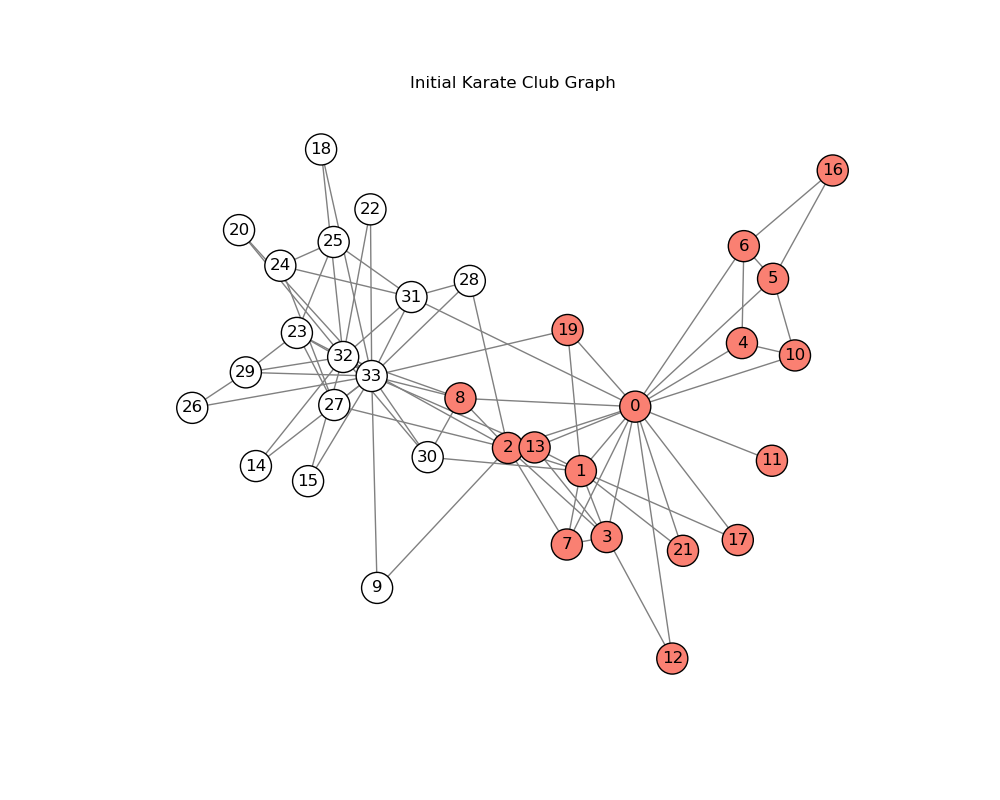
\includegraphics[width=1\linewidth]{initial_karate_club_graph.png}
    \caption{Initial Karate Club Graph)}
    \label{fig:initial}
\end{figure}

The Girvan-Newman algorithm is iterative, repeatedly removing edges with the highest betweenness centrality until the graph is split into disconnected components. For each iteration, an image is generated to visualize the split. The last generated image visualizes the split into disconnected components. See Figure \ref{fig:iteration_11}.

The below code runs the Girvan-Newman algorithm:
\begin{lstlisting}
while nx.number_connected_components(working_graph) == 1:
    edge_betweenness = nx.edge_betweenness_centrality(working_graph)
    edge_to_remove = max(edge_betweenness, key=edge_betweenness.get)
    working_graph.remove_edge(*edge_to_remove)

    if nx.number_connected_components(working_graph) > 1:
        break

    save_graph_snapshot(...)

    iteration += 1    
\end{lstlisting}

\begin{figure}
    \centering
    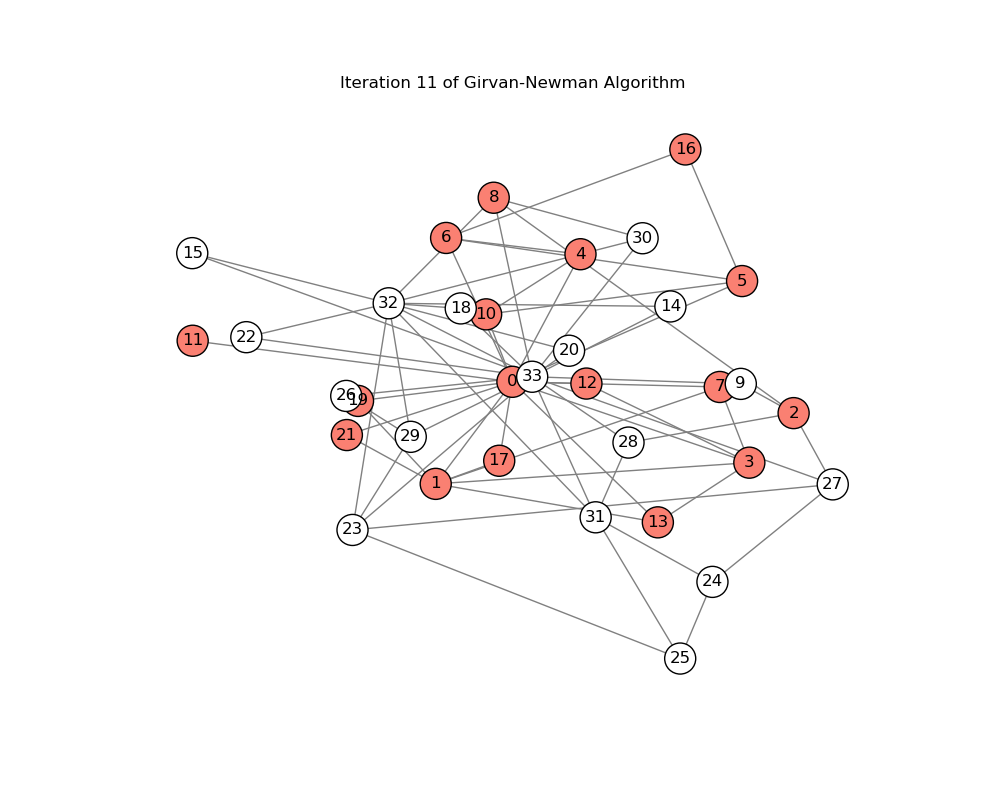
\includegraphics[width=1\linewidth]{iterations/girvan_newman_iteration_11.png}
    \caption{Girvan Newman Iteration 11}
    \label{fig:iteration_11}
\end{figure}

\emph{Q: How many iterations did it take to split the graph?}

It took 11 iterations to split the graph with the Girvan-Newman algorithm.

% --------------- Q3 --------------- %

\section*{Q3}

Below are the results of the comparison between the connected components of the Girvan-Newman split graph (Q2) with the connected components of the actual split Karate club graph (Q1):

\begin{lstlisting}
Actual split factions:
Mr. Hi's faction: {0, 1, 2, 3, 4, 5, 6, 7, 8, 10, 11, 12, 13, 16, 17, 19, 21}
John's faction: {32, 33, 9, 14, 15, 18, 20, 22, 23, 24, 25, 26, 27, 28, 29, 30, 31}

Comparison of Girvan-Newman results with actual split:
Component 1: {0, 1, 3, 4, 5, 6, 7, 10, 11, 12, 13, 16, 17, 19, 21}
Matches actual factions? No, not matched
Component 2: {2, 8, 9, 14, 15, 18, 20, 22, 23, 24, 25, 26, 27, 28, 29, 30, 31, 32, 33}
Matches actual factions? No, not matched
\end{lstlisting}

I extracted the actual factions based on each node's attribute 'club', creating sets for the "Mr. Hi" and "John" factions.

The program's code compares the Girvan-Newman split components with the actual components to determine whether they match, then outputs "matched" or "not matched" accordingly.

\emph{Q: Did all of the same colored nodes end up in the same group? If not, what is different?}

No, not all nodes from the same faction ended up in the same group. Two of Mr. Hi's faction nodes were grouped with John's in the final split (Refer to Figure \ref{fig:iteration_11}). 

% --------------- References --------------- %

\clearpage

\section*{References}

\begin{itemize}
    \item {Centrality - NetworkX, \url{https://networkx.org/documentation/stable/reference/algorithms/centrality.html}}
    \item {Components - NetworkX, \url{https://networkx.org/documentation/stable/reference/algorithms/component.html}}
    \item{CS 432/532 - NetworkX Example, \url{https://github.com/odu-cs432-websci/public/blob/main/432_NetworkX_example.ipynb}}
    \item {Drawing - NetworkX, \url{https://networkx.org/documentation/stable/reference/drawing.html#module-networkx.drawing.layout}}
    \item {Karate Club - NetworkX, \url{https://networkx.org/documentation/stable/auto_examples/graph/plot_karate_club.html}}
    \item{Tutorial - NetworkX, \url{https://networkx.org/documentation/stable/tutorial.html}}
\end{itemize}

\end{document}

